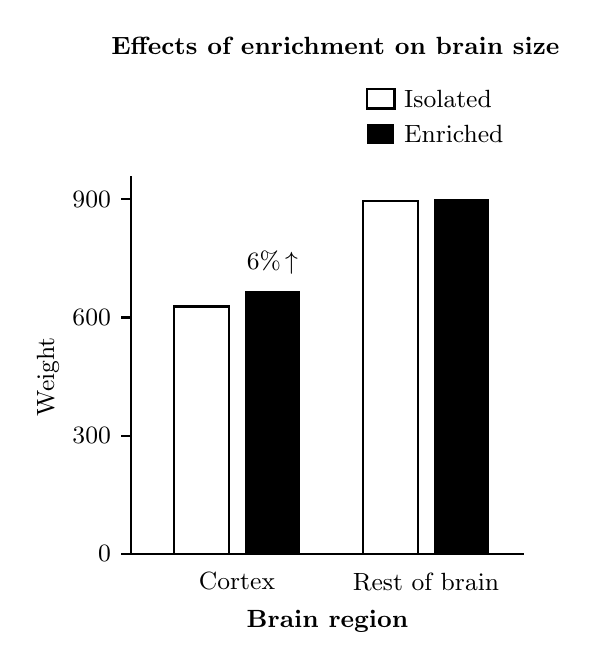
\begin{tikzpicture}[x=1cm,y=0.005cm,font=\small]
% title and legend
\node[font=\small\bfseries] at (2.6,1290) {Effects of enrichment on brain size};
\draw[thick] (3.0,1130) rectangle (3.35,1180);
\node[right] at (3.35,1155) {Isolated};
\fill[black] (3.0,1040) rectangle (3.35,1090);
\node[right] at (3.35,1065) {Enriched};
% axes
\draw[thick] (0,0) -- (5.0,0);
\draw[thick] (0,0) -- (0,960);
\foreach \v in {0,300,600,900} {
  \draw[thick] (0,\v) -- (-0.12,\v) node[left] {\v};
}
\node[rotate=90] at (-1.05,450) {Weight};
% cortex
\draw[thick] (0.55,0) rectangle (1.25,628);
\fill[black] (1.45,0) rectangle (2.15,667);
\node at (1.8,740) {6\%\,$\uparrow$};
% rest of brain
\draw[thick] (2.95,0) rectangle (3.65,896);
\fill[black] (3.85,0) rectangle (4.55,901);
% category labels
\node at (1.35,-70) {Cortex};
\node at (3.75,-70) {Rest of brain};
\node[font=\small\bfseries] at (2.5,-170) {Brain region};
\end{tikzpicture}
